\documentclass[a4,semhelv,semrot,landscape]{seminar}
\usepackage[dvips]{graphicx}
\usepackage{fancybox}
\usepackage{a4wide}
\usepackage{amsmath}
\usepackage{amsxtra}

\newcommand{\mb}[1]{\mathbf{#1}}
\newcommand{\ket}[1]{|#1 \rangle}
\newcommand{\bra}[1]{\langle #1|}
\newcommand{\Alpha}{\bar{\alpha}}
\newcommand{\Exp}[2]{e^{i \mb{#1} \cdot \mb{#2} }}
\newcommand{\ExpM}[2]{e^{-i \mb{#1} \cdot \mb{#2} }}
\newcommand{\state}[2]{\psi_{#1 #2}}
\newcommand{\Muq}{\mu(\mb{q},\theta,\phi)}
\newcommand{\Angstrom}{\stackrel{\circ}{\mathrm{A}} }
\newcommand{\InvAngstrom}{ \stackrel{\circ}{\mathrm{A}}^{-1} } 
\newcommand{\Half}{\frac{1}{2}}

\slideframe{shadow}

\newcommand{\heading}[1]{ \begin{center}%
                          {\large {\bf \sffamily{#1}}}\\[3mm]%
                          \hrule\vspace{1mm}
                          \end{center}}
\sffamily

\begin{document}

\begin{slide}
    \begin{center}
    
\includegraphics[width=1.5cm]{UMCrest97.eps}\\[5mm]
    {\bf \Large INVESTIGATION OF\\ THEORETICAL APPROACHES FOR 
    COMPUTING RELATIVISTIC ATOMIC FORM FACTORS}\\[5mm]
    \hrule
    \vspace{5mm}
    {\large Michael Papasimeon \\
    Supervisor : Dr. Christopher Chantler \\
    Optics Group, School of Physics \\
    The University of Melbourne}
    \end{center}
\end{slide}

\begin{slide}
    \heading{EXAMPLES OF USEFULNESS OF ATOMIC FORM FACTORS: $f$}
    \begin{itemize}
        \item Crystallography: Structure Factors
        \[
            F(hkl) = \sum_j f_j e^{-M_j} 
                      e^{2\pi i (hx_j + ky_j + lz_j) }
        \]
        \item Materials Science: Optical Properties of Materials   \\ 
              (Refractive Index $n_r$ and Dielectric Constant $\epsilon$)
        \[
           n_r = n+ik = \sqrt{\epsilon} = 1 - \delta - i\beta
               = 1 - \frac{r_0}{2\pi} \lambda^2
                 \sum_j n_j f_j
        \]
        \item Applications in X Ray Optics\\
              Including experimental work undertaken in School of Physics 
              X Ray lab
    \end{itemize}
\end{slide}

\begin{slide}
    \heading{THE ATOMIC FORM FACTOR $f$: WHAT IS IT?}
    \begin{center}
    Photon-Atom interactions are described by QFT.\\
    $f = f_0 + f' + if''$ 
        \begin{tabular}{|c|c|c|} \hline
        $f_0(q)$ & $f'(\omega)$ & $f''(\omega)$ \\ \hline
        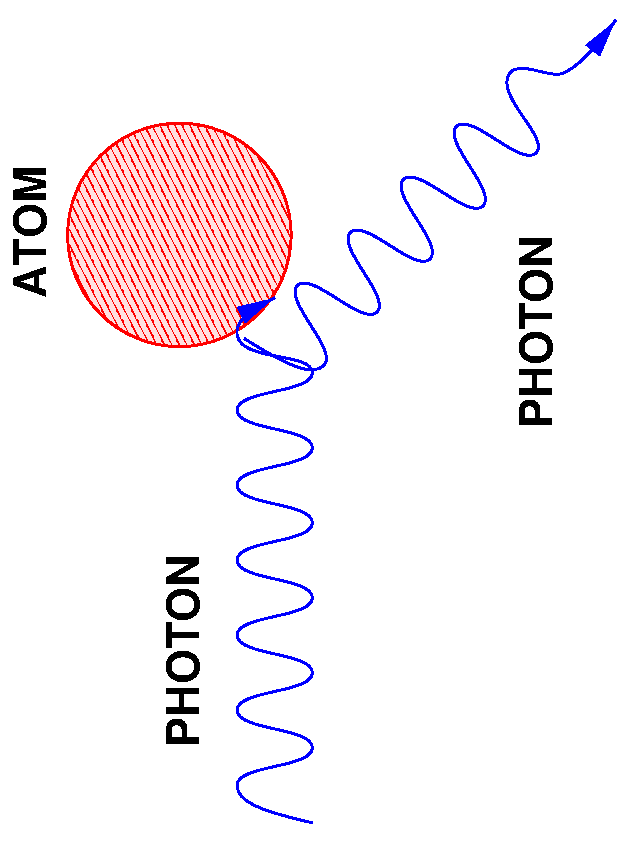
\includegraphics[angle=-90,width=3.2cm]{f0.eps}  &   
        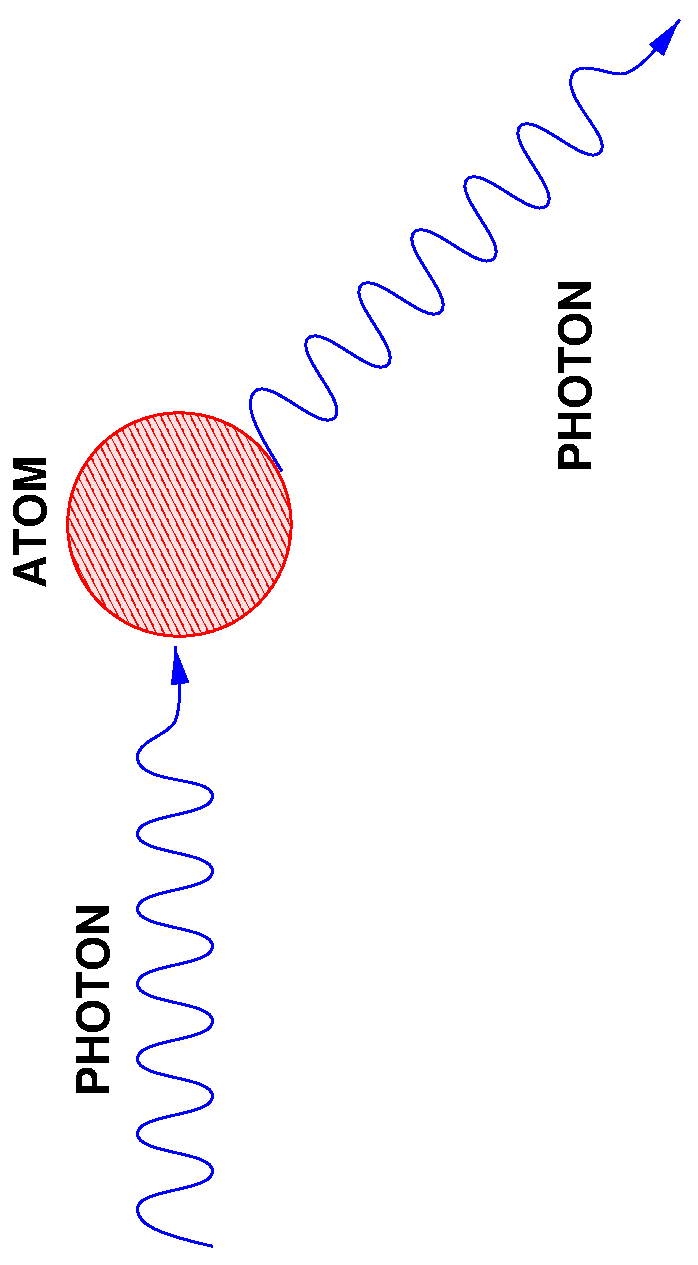
\includegraphics[angle=-90,width=3.2cm]{fprime.eps}  & 
        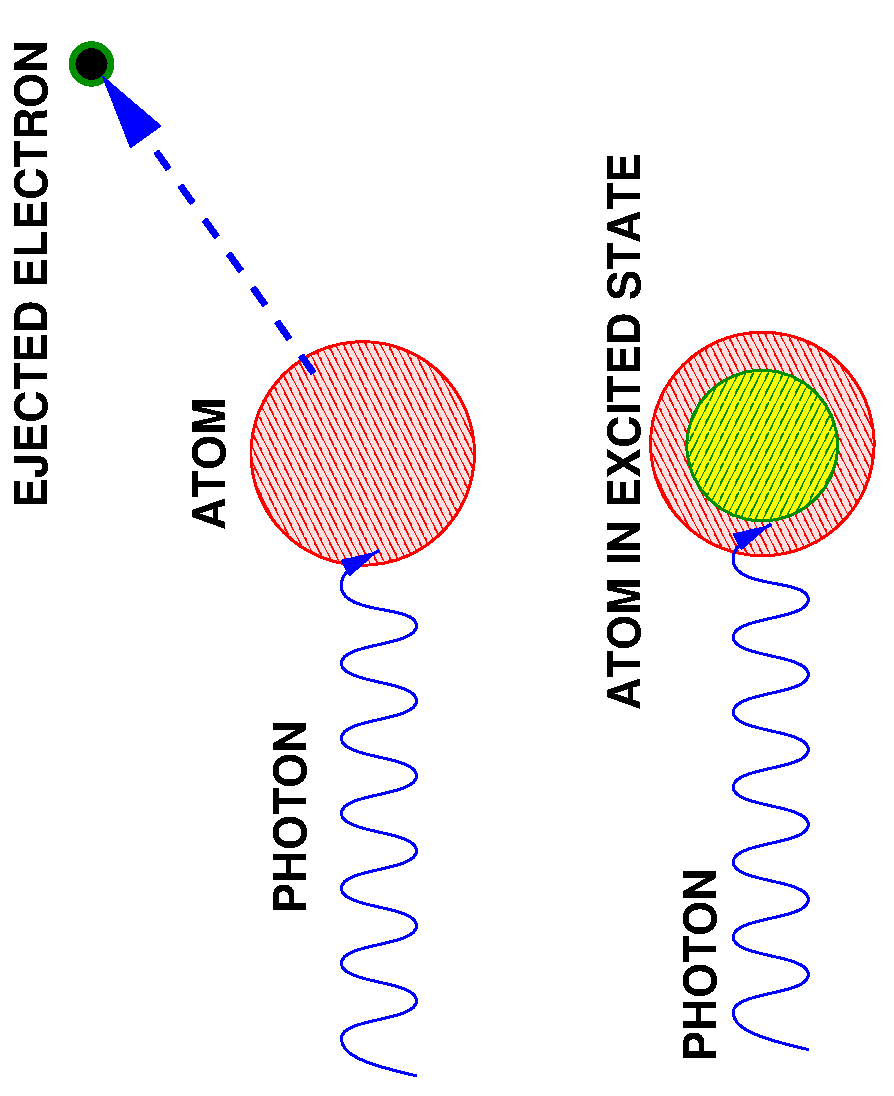
\includegraphics[angle=-90,width=3.2cm]{fdoubleprime.eps} \\ \hline
        NORMAL & ANOMALOUS & ANOMALOUS  \\ \hline
        \end{tabular}
    \end{center}
\end{slide}

\begin{slide}
    \heading{HOW DO WE CALCULATE $f = f_0+f'+if''$ ?}
    \begin{itemize}
        \item {\bf NORMAL FORM FACTOR:} The scattering power of an atom
              relative to the scattering power of a free electron.
        \[
             f_0(q) = \int \rho(\mb{r}) e^{i\mb{q}\cdot\mb{r}} \; d\mb{r}
        %\]
        \; \; \; \; \; \; ; \; \; \; \; \; \;  
        %\[
            q = |\mb{k_{f}} - \mb{k_{i}}| = \frac{4\pi \sin(\theta/2)}{\lambda}
            \InvAngstrom
        \]
        \item {\bf IMAGINARY COMPONENT OF ANOMALOUS FORM FACTOR:}
        Related to the total photoionisation cross section $\sigma(\omega)$.
        ($r_0 = e^2 / mc^2$)
        \[
             f''(\omega) = \frac{\omega}{4\pi c r_0} \sigma(\omega)
        \]
        \item {\bf REAL COMPONENT OF ANOMALOUS FORM FACTOR:} 
              $f'(\omega)$ can be calculated from $f''(\omega)$
              using a Kramers-Kronig dispersion relation.
    \end{itemize}
\end{slide}

\begin{slide}
    \heading{THEORETICAL LIMITATIONS AND ASSUMPTIONS}
    \begin{itemize}
        \item Isolated Atom
        \item Electromagnetic Field: Classical.
                Electric Dipole, Electric Quadrupole, \\ 
                All Poles, RMP
        \item Atomic Structure: Schr\"odinger, Dirac
        \item Perturbation Theory: 1st order relativistic, S-Matrix (QFT)
        \item Numerical and Computational Issues: singularities, convergence
    \end{itemize}
\end{slide}


\begin{slide}
    \heading{PROJECT AIM AND RESULTS}
    \begin{center}
    {\it {\bf AIM:} Investigate the issues, assumption and limitations 
         in atomic form factor theory by a critical analysis and study of 
         hydrogenic atoms}
    \end{center}
    \begin{itemize}
         \item New analytic result for relativistic normal form factor
         \item New semi analytic results for first and second order 
                  photoionisation amplitudes.
          \item New numerical results for $f''(\omega)$ using S-matrix
                  theory and relativistic perturbation theory.
          \item Calculated bound-bound relativistic transition 
                  amplitudes for the first three
                  excited states for hydrogenic atoms.
          \item Angular dependent results
    \end{itemize}
\end{slide}

\begin{slide}
    \heading{NORMAL FORM FACTOR $f_0(q)$ FOR HYDROGENIC ATOMS \\
             ANGULAR DEPENDENT CONTRIBUTION}
    \begin{itemize}
        \item ANALYTIC NON RELATIVISTIC RESULT (has been done before)
        \[
             f_0(q) = \left( \frac{2Z}{a_0} \right)^4 
                     \left[ \left( \frac{2Z}{a_0} \right)^2 + q^2 \right]^{-2} 
        \]
        \item {\bf NEW} ANALYTIC RELATIVISTIC RESULT 
        \[
        \boxed{
              f_0(q) = 
            \frac{\Gamma(2\gamma_1)}{2iq \Gamma(2\gamma_1+1)}
            \left(
                \frac{2Z}{a_0}
            \right)^{2\gamma_1 + 1} 
            \left[
                \frac{
                    \left(
                        \frac{2Z}{a_0} + iq
                    \right)^{2\gamma_1}
                    -
                    \left(
                        \frac{2Z}{a_0} - iq
                    \right)^{2\gamma_1}
                } {
                    \left[
                        \left(
                            \frac{2Z}{a_0} 
                        \right)^2   
                        + q^2
                    \right]^{2\gamma_1}
                }
            \right]
        }
        \]
        \item $\gamma_1 = \sqrt{1 - (\alpha Z)^2}$, 
        $\alpha = $ fine structure constant,\\ $a_0 = $ Bohr radius,
        $Z = $ Atomic Number. For low Z, $\gamma_1 \approx 1$.
    \end{itemize}
\end{slide}

\begin{slide}
    \heading{ATOMIC HYDROGEN}
    \begin{center}
        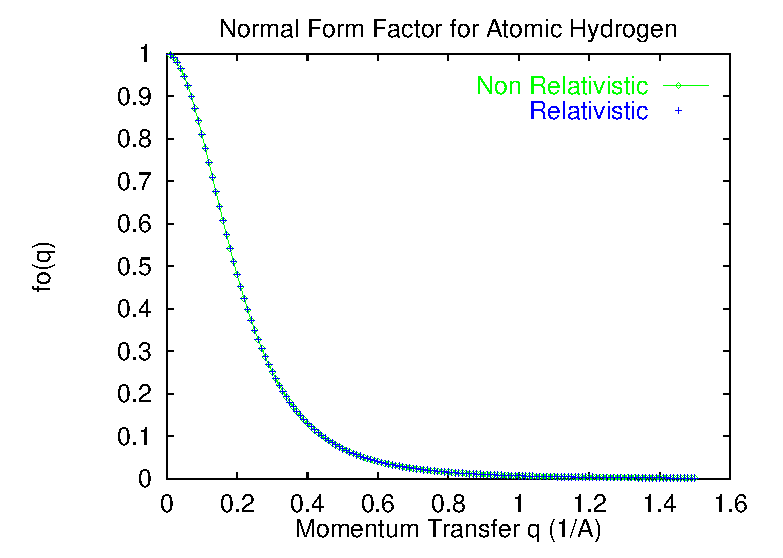
\includegraphics[width=5.3cm]{f0_hydrogen.eps}
        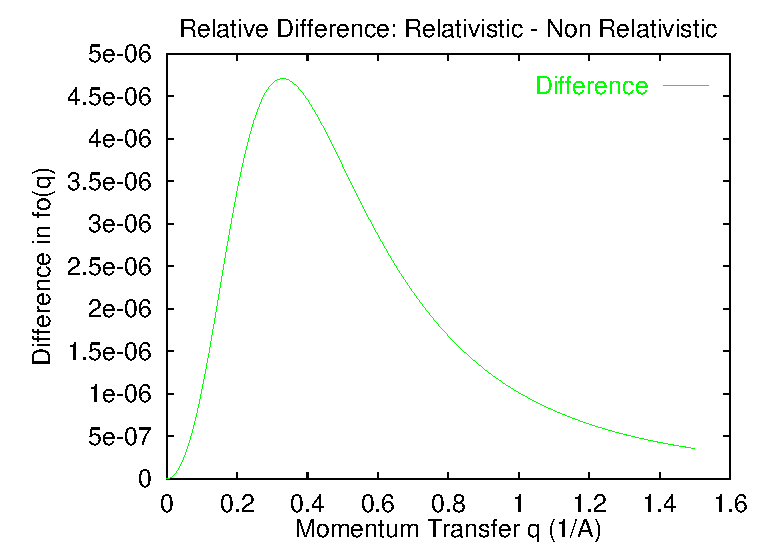
\includegraphics[width=5.3cm]{delta_theory.eps}
    \end{center}
    \begin{itemize}
        \item Approximately 0.015\% difference between reltativistic
              and non relativistic results.
        \item Current experimental precision: 0.1\% -- 1\%
    \end{itemize}
\end{slide}

\begin{slide}
    \heading{HYDROGENIC URANIUM}
    \begin{center}
        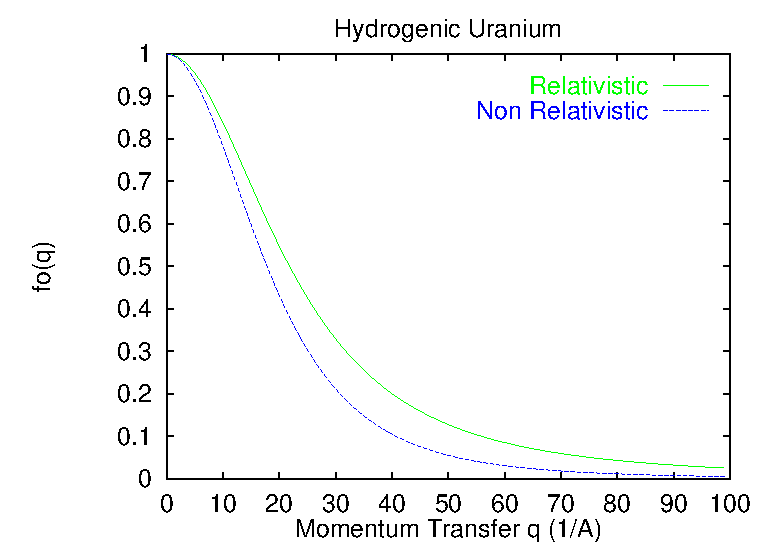
\includegraphics[height=6.5cm]{f0_uranium.eps}
    \end{center}
\end{slide}

\begin{slide}
    \heading{PHOTOIONISATION COORDINATE SYSTEM}
    \begin{center}
        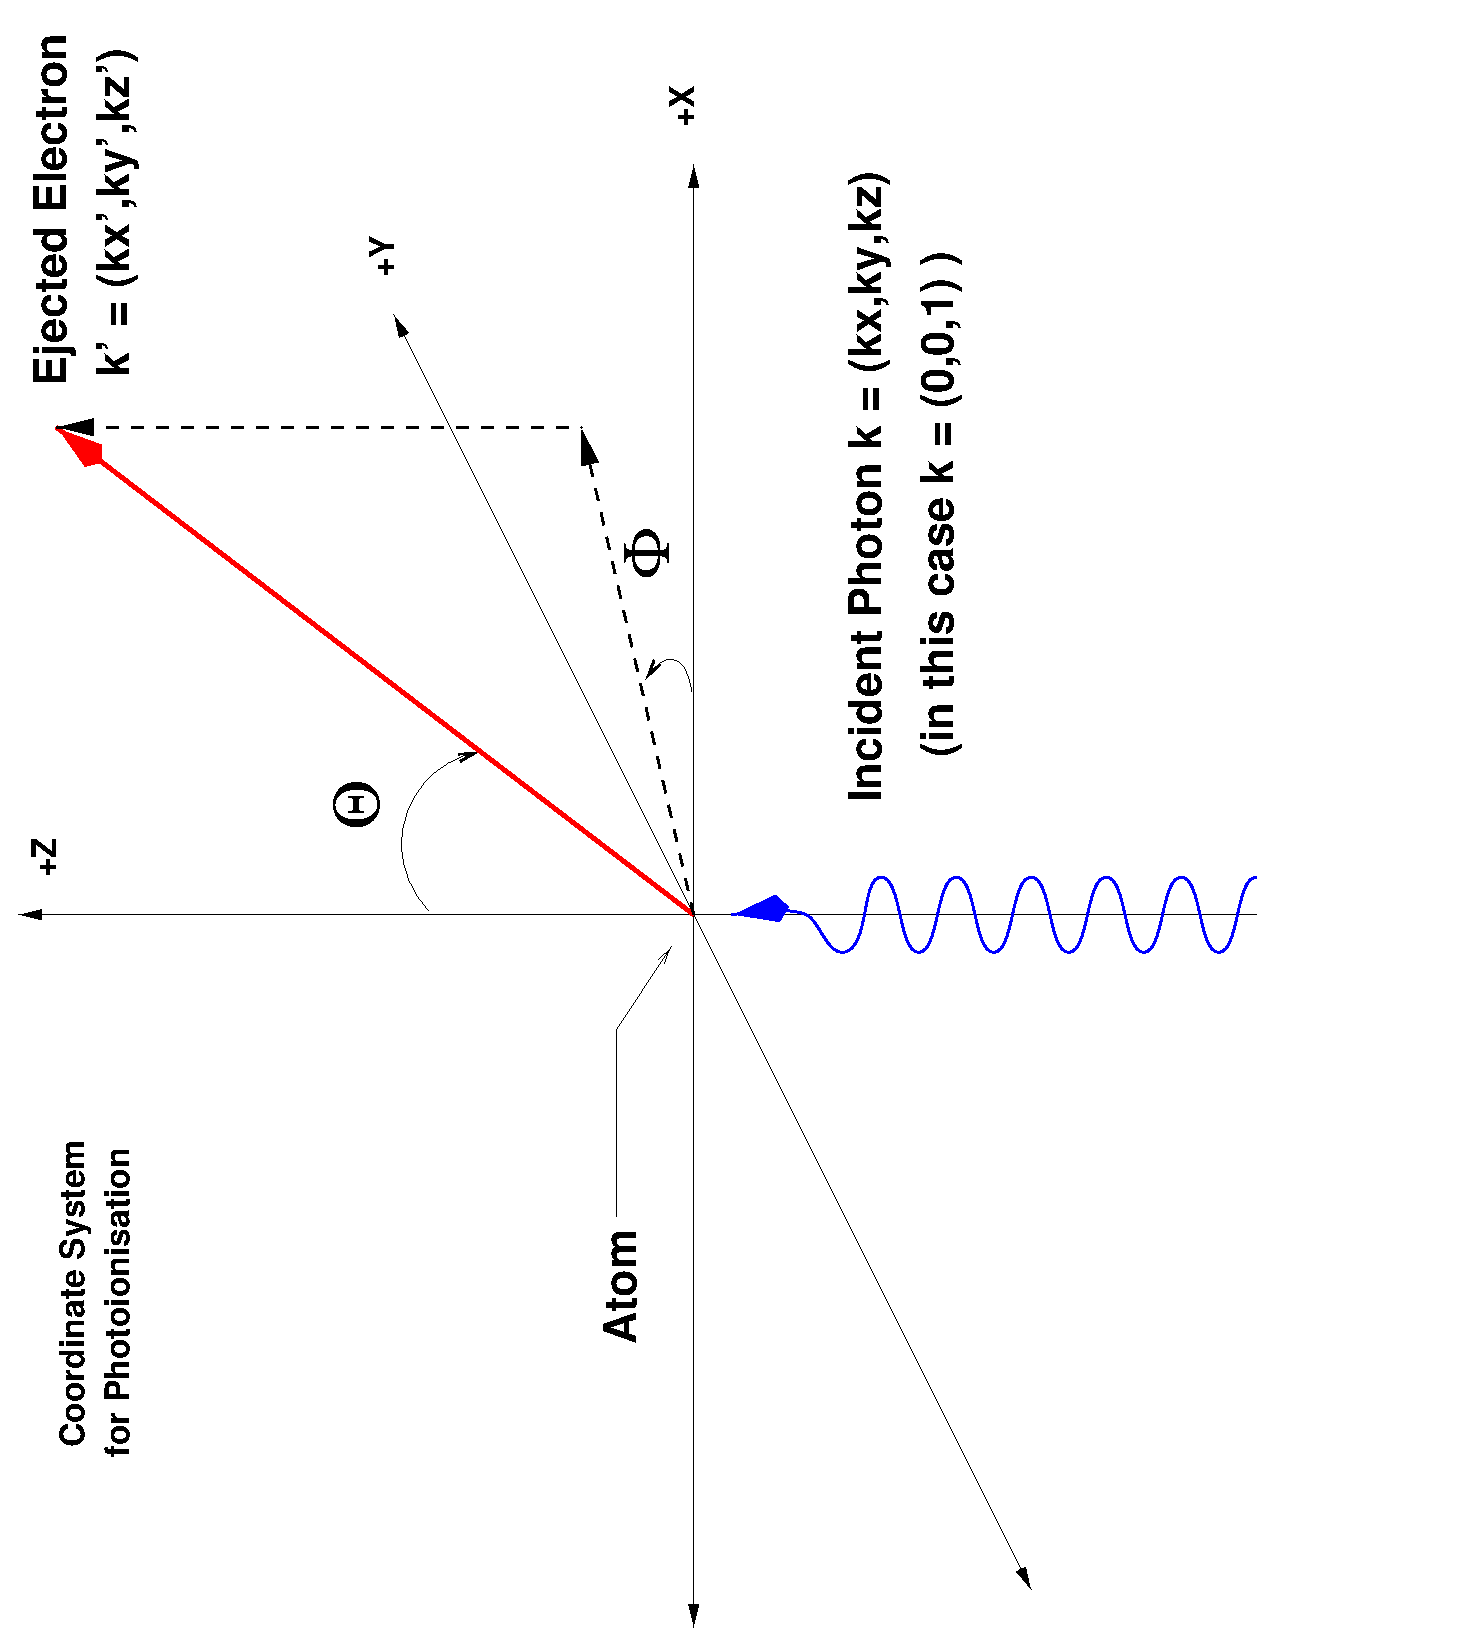
\includegraphics[width=6.0cm,angle=-90]{coords.eps}
        \[
            k'_x  =  |k'| \sin(\Theta) \cos(\Phi) \; ,
            k'_y  =  |k'| \sin(\Theta) \sin(\Phi) \; ,
            k'_z  =  |k'| \cos(\Theta)
        \]
    \end{center}
\end{slide}

\begin{slide}
    \heading{IMAGINARY ANOMALOUS ATOMIC FORM FACTOR $f''(\omega)$}
    \begin{itemize}
        \item {\bf APPROACHES TO CALCULATING} $f''(\omega)$: 
            Standard Perturbation Theory,
            Relativistic Perturbation Theory,
            Relativistic S-Matrix Theory
        \item {\bf RELATIVISTIC PHOTON ABSORPTION AND EMISSION OPERATORS (QFT)}
        \[
            \mathcal{A}_i  =  \sum_j \Alpha \cdot \hat{\epsilon}_j \Exp{k_i}{r_j} 
            \hspace{1.5cm}
            \mathcal{A}_f^{\dag}  =  \sum_j \Alpha \cdot \hat{\epsilon}_j \ExpM{k_f}{r_j}
        \]
        Sum over $j$ electrons, $\Alpha$ = Dirac alpha matrix,
        $\hat{\epsilon}_j$ = photon polarisation, \\
        $\mb{k}$ = photon wavevector, $\mb{k'}$ = ejected electron
        wave vector, $r_j$ = coordinate of $j$-th electron.
        \item {\bf RELATIVISTIC PHOTOIONISATION AMPLITUDE: HYDROGEN}
        \[
            A_1(\mb{k},\mb{k'}) = \bra{\psi_c} \mathcal{A}_i \ket{\psi_0} = \bra{\psi_c} \Exp{k}{r} \Alpha_j \ket{\psi_0}
        \]
    \end{itemize}
\end{slide}

\begin{slide}
    \heading{ALL POLES AND ELECTRIC DIPOLE RESULTS}
    \begin{multline*}
     A_1(\mb{k},\mb{k'})_{\binom{x}{y}} =  
    \frac{G_0 \Gamma(\gamma_1 + 2)}{\sqrt{4\pi}}  \times \\
    \int_{0}^{2\pi}
    \int_{0}^{\pi} 
        \left[
            \frac {
            \binom{1}{i}
            \sin(\theta) [ \xi(k'_x - ik'_y) \pm i F_0 \sin(\theta) e^{i\phi} ]
            } {
                (\frac{1}{2}\sigma_1 - i \Muq )^{\gamma_1 + 2}
            }
       \right]
    \; d\theta
    \; d\phi
    \end{multline*}
    \[
        A_1^{E1}(\mb{k},\mb{k'})_j = A_1(0,\mb{k'})_j
    \]
    \[
        \Muq = q_x \sin\phi \cos\theta + 
               q_y \sin\phi \sin\theta +
               q_z \cos\phi
    \]
\end{slide}

\begin{slide}
    \heading{THE FORWARD SCATTERING DIRECTION}
    \begin{multline*}
     A_1(k,k')_x  =  \frac{\pi}{\sqrt{\pi}}  
                        \left( \frac{2Z}{a_0} \right)^{3/2}
                        \sqrt{ \frac{1 - \epsilon_1}{
                                    2 \Gamma(2\gamma_1 + 1)
                               } } \times \\
     \Biggl[
        \left( \frac{Z}{a_0} \right)^{-(\gamma_1 + 2)}
    \Gamma(\gamma_1 + 2)
    \; _2 F_1 \left(
                \frac{\gamma_1 + 2}{2} ,
                \frac{\gamma_1 + 3}{2} ;
                1 ;
                - \left(
                    \frac{2a_0}{Z}
                \right)^2
                (k - k')^2
           \right)
    \\ + 
    \frac{1}{8} (k - k')^2 
    \left( \frac{Z}{a_0} \right)^{-(\gamma_1 + 4)}
    \Gamma(\gamma_1 + 4) \times \\
    \; _2 F_1 \left(
                \frac{\gamma_1 + 4}{2} ,
                \frac{\gamma_1 + 5}{2} ; 
                1 ;
                - \left( \frac{2a_0}{Z} \right)^2
                (k - k')^2
            \right)
    \Biggr]
    \end{multline*}
    \[
         A_1(k,k')_y = -i A_1(k,k')_x \;\;\;\; ; \;\;\;\; 
         |A_1(k,k')_y|^2 = |A_1(k,k')_x|^2
    \]
\end{slide}

\begin{slide}
    \heading{RELATIVISTIC S-MATRIX THEORY APPLIED TO \\ ATOMIC FORM FACTOR CALCULATIONS}
    \[
        \mathrm{Im} A_2(\omega) = r_0 f''(\omega) = \frac{\omega}{4 \pi c} \sigma^{TOT}(\omega)
    \]
    \[
          A_2 = 
     -r_0 mc^2 \sum_p
     \left[
     \frac{
        \bra{m} \mathcal{A}_f^\dag \ket{p}
        \bra{p} \mathcal{A}_i \ket{n}
     }{
        E_n - E_p + \hbar\omega_f + i0_+
     }
     +
     \frac{
        \bra{m} \mathcal{A}_i \ket{p}
        \bra{p} \mathcal{A}_f^\dag \ket{n}
     }{
        E_n - E_p - \hbar\omega_i + i0_+
     }
     \right]
    \]
    \begin{multline*}
         A_2^R(\omega) = A_2(\mb{k},\mb{k'})_j = 
         -r_0 mc^2  
%        \left[
        \int_0^\infty
             \frac{
             | A_1(\mb{k},\mb{k'})_j |^2
        }{
            E_0 - E_c + \hbar\omega + i0_+
        } 
        dE_c \\
        - r_0 mc^2
        \int_0^\infty
        \frac{
            |A_1(\mb{-k},\mb{k'})_j |^2
        }{
           E_0 - E_c - \hbar\omega - i0_+
        }
        dE_c
%        \right]
    \end{multline*}
    \[
        A_2^{E1}(\mb{k},\mb{k'})_j  = A_2(0,\mb{k'})_j 
    \]
\end{slide}

\begin{slide}
    \heading{NUMERICAL CALCULATIONS}
    \begin{itemize}
        \item Approximately 5000 lines of C++ 
        \item Approximately 2000 lines of Mathematica
        \item Quadrature Methods
            \begin{itemize}
                \item Simpson, Trapezoidal
                \item Gauss-Legendre (10 point)
                \item Converging Romberg
            \end{itemize}
        \item Intensive/Expensive Computation: Triple Integrals $\theta$,$\phi$, and Energy
        \item Singularities, open interval and numerical
              Cauchy Principal value integrations
        \item Parameters: Bound-Bound $i0_+ = i\frac{\Gamma}{2}$ \\
                          Continuum $i0_+$ = small value.
    \end{itemize}
\end{slide}

\begin{slide}
    \heading{RESULTS - ALL POLES AND ELECTRIC DIPOLE} 
    \begin{center}
        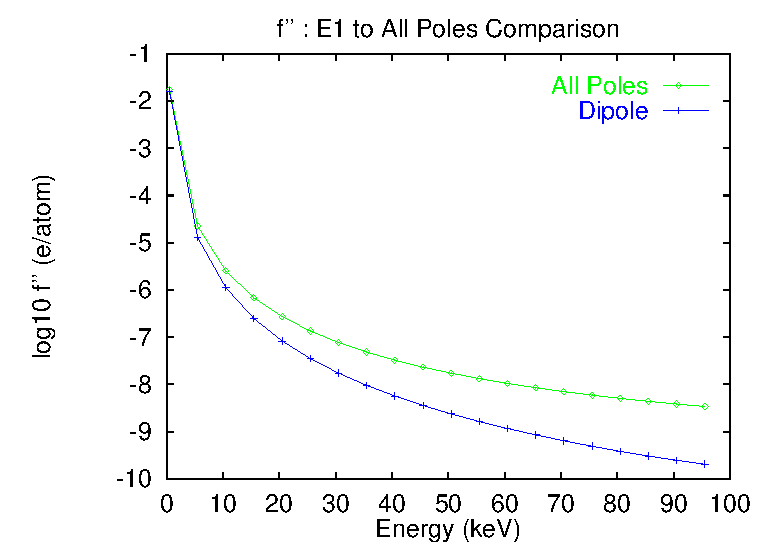
\includegraphics[width=9.5cm]{compare_poles_1.eps}
    \end{center}
\end{slide}

\begin{slide}
    \heading{COMPARISON: CHANTLER (BOUND H), KISSEL (ATOMIC H)} 
    \begin{center}
        \includegraphics[width=9.5cm]{all_compare.eps}
    \end{center}
\end{slide}

\begin{slide}
    \heading{CONCLUSIONS AND FURTHER WORK}
    \begin{itemize}
    \item Summary of Results: Hydrogenic Atoms
        \begin{itemize}
            \item New analytic result for relativistic normal form factor
            \item New Semi analytic results for first and second order 
                  photoionisation amplitudes.
            \item New Numerical results for $f''(\omega)$ using S-matrix
                  theory and relativistic perturbation theory.
            \item Calculated bound-bound relativistic transition 
                  amplitudes for the first three
                  excited states for hydrogenic atoms.
            \item Angular dependent results
        \end{itemize}
    \item Further Work:
        Refine convergence,
        develop relativistic perturbation theory
        computation of $f'(\omega)$,
        XAFS (X Ray Anomalous Fine Structure) - multiple
              scattering processes off multiple atoms (eg: molecular 
              hydrogen).
    \end{itemize}
\end{slide}

\begin{slide}
    \begin{center}
        {\bf {\Huge QUESTIONS?}} \\[5mm] \hrule
    \end{center}
\end{slide}

\end{document}


